Since haptic is one of the types of information that a BVI user can rely on, it was a good idea to test haptic devices in the experiment. These haptic devices would not detect the real object per se, but would receive the information from Unity3D based on the position of the user inside the virtual environment.
 
 The virtual cane was a simple development, since the controller already had a vibration motor inside of it. Knowing that, was only a matter to find the right commands and write an algorithm that worked. A pseudo-code is presented at Appendix \ref{ap:virtual_apend}. The two differences between the virtual cane and the haptic belt are the command to check the distance and the fact that with the cane the user must point to the direction where he/she wants to investigate if there is an obstacle whilst the belt indicates to the user the direction of the closest object.
 
 The idea to design a haptic belt came as a suggestion from one of the research members. It was possible to buy one directly from the internet but the cost was too high, so it was decided to assemble one from scratch. The project was based on a haptic compass \cite{kylecorry31_instructables_2020}, but instead of having the input being made by a magnetometer, it was made by the Unity3D.
 
 The first prototype was made using a Arduino Mega 2560, LEDs and a protoboard. If Unity3D could send a command to turn the LED on, then the software would be able to do the same with a coin vibrator. After checking the communication between Unity3D and Arduino, it was time to build the proper belt.
 
 The materials used were:
 \begin{itemize}
     \item DOIT ESP32 DevKit v1. (Datasheet in the Annex \ref{an:esp32_annex});
     \item A printed circuit board (PCB)
     \item A leather belt;
     \item 8 Coin Vibrator 1027;
     \item 16 female P2 jacks or PJ-320B;
     \item 16 P2 male or PJ cable connectors;
     \item 8 straps;
     \item Duct tape;
     \item A 3D printed case.
 \end{itemize}
 
 The first step was to correct and adapt the algorithm used on the Arduino to be used on ESP32 also using the LEDs. After it was made sure that it would also work with an ESP32, the system was designed on the EasyEDA website \cite{easyeda} them a PCB was ordered with the schematic presented in the Appendix \ref{ap:haptic_apend}. While the PCB didn't arrive the coin vibrator and the cables were being soldered. When the PCB arrived, it was time to solder the board P2 jacks and design a case for it, represented in the Figure \ref{fig:case_cinto}. After everything was soldered, printed, and connected it was ready, as is represented in the Figure \ref{fig:cinto_haptico}.
 
 \begin{figure}[!htb]
     \centering
     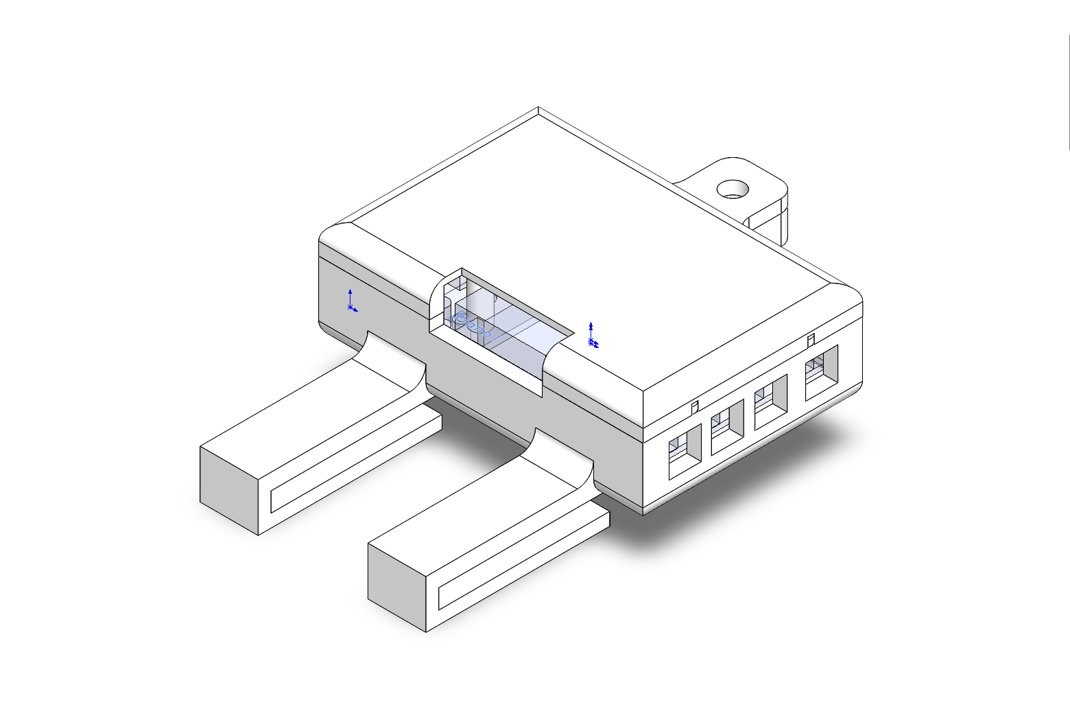
\includegraphics[width = 0.8\linewidth]{Cinto/Case Cinto.png}
     \caption{CAD model of the designed case}
     \label{fig:case_cinto}
 \end{figure}
 \begin{figure}[!htb]
     \centering
     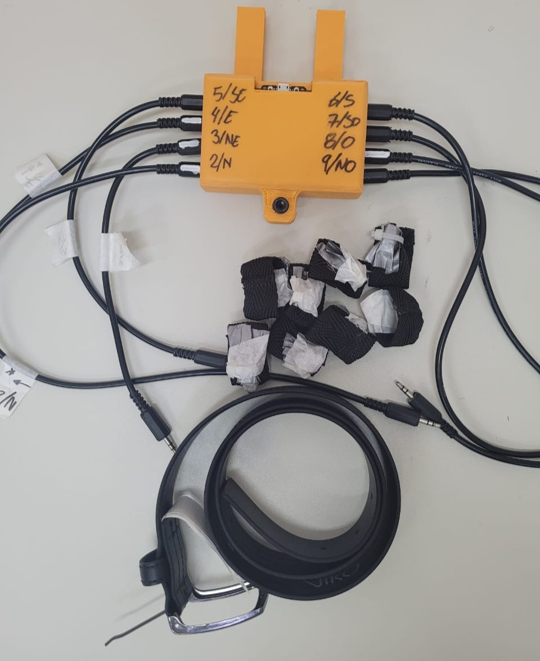
\includegraphics[width = 0.8\linewidth]{Cinto/Cinto Haptico.png}
     \caption{Haptic belt}
     \label{fig:cinto_haptico}
 \end{figure}
 
 Until this moment the belt was working cabled, but since the participant could walk great distances it was decided that the correct way to connect Unity3D with the ESP32 would be by wireless and it was decided to use a Bluetooth connection. The pseudo-code used in the development are in the Appendix \ref{ap:haptic_apend}.
